%%%%%%%%%%%%%%%%%%%%%%%%%%%%%%%%%%%%
% Alexander Powell
% CSCI 524 - Computer Architecture
% Prof: Adwait Jog
% Homework #8
% Due: 12.02.2016
%%%%%%%%%%%%%%%%%%%%%%%%%%%%%%%%%%%%

\documentclass[10pt]{article} %
\usepackage{fullpage}
\usepackage{graphicx}
\usepackage{graphics}
\usepackage{psfrag}
\usepackage{amsmath,amssymb}
\usepackage{enumerate}
\usepackage{pdfpages}

\setlength{\textwidth}{6.5in}
\setlength{\textheight}{9in}

\newcommand{\cP}{\mathcal{P}}
\newcommand{\N}{\mathbb{N}}
\newcommand{\Z}{\mathbb{Z}}
\newcommand{\R}{\mathbb{R}}
\newcommand{\Q}{\mathbb{Q}}
\newcommand{\points}[1]{{\it (#1 Points)}}
\newcommand{\tpoints}[1]{{\bf #1 Total points.}}

\title{CSCI 524 -- Computer Architecture \\
Homework 8 \\
{\large{\bf Due: December 2, 2016}}}
\date{}
\author{Alexander Powell}


\begin{document}
\maketitle
\begin{enumerate}[1.]
\item %1
\textbf{Problem 6.3 from COD reference ($5^{\text{th}}$ Edition).  }

\begin{itemize}

\item
\textbf{6.3.1}

Actually, a sequential binary search alreaady has a pretty good execution time because the array is assumed to be in order so the algorithm can just keep dividing it into smaller halves until the desired element is found.  Therefore, it has a time complexity of $\log_2 N$ in the worst case which is far less than $N$.  While probably unnecessary, the computation of low and high can be computed on one core, mid can be computed on a second, and the comparison can be computed on a third.  After three cores, there should be no observable speedup.  A graph of this behavior would look something like:

\begin{center}
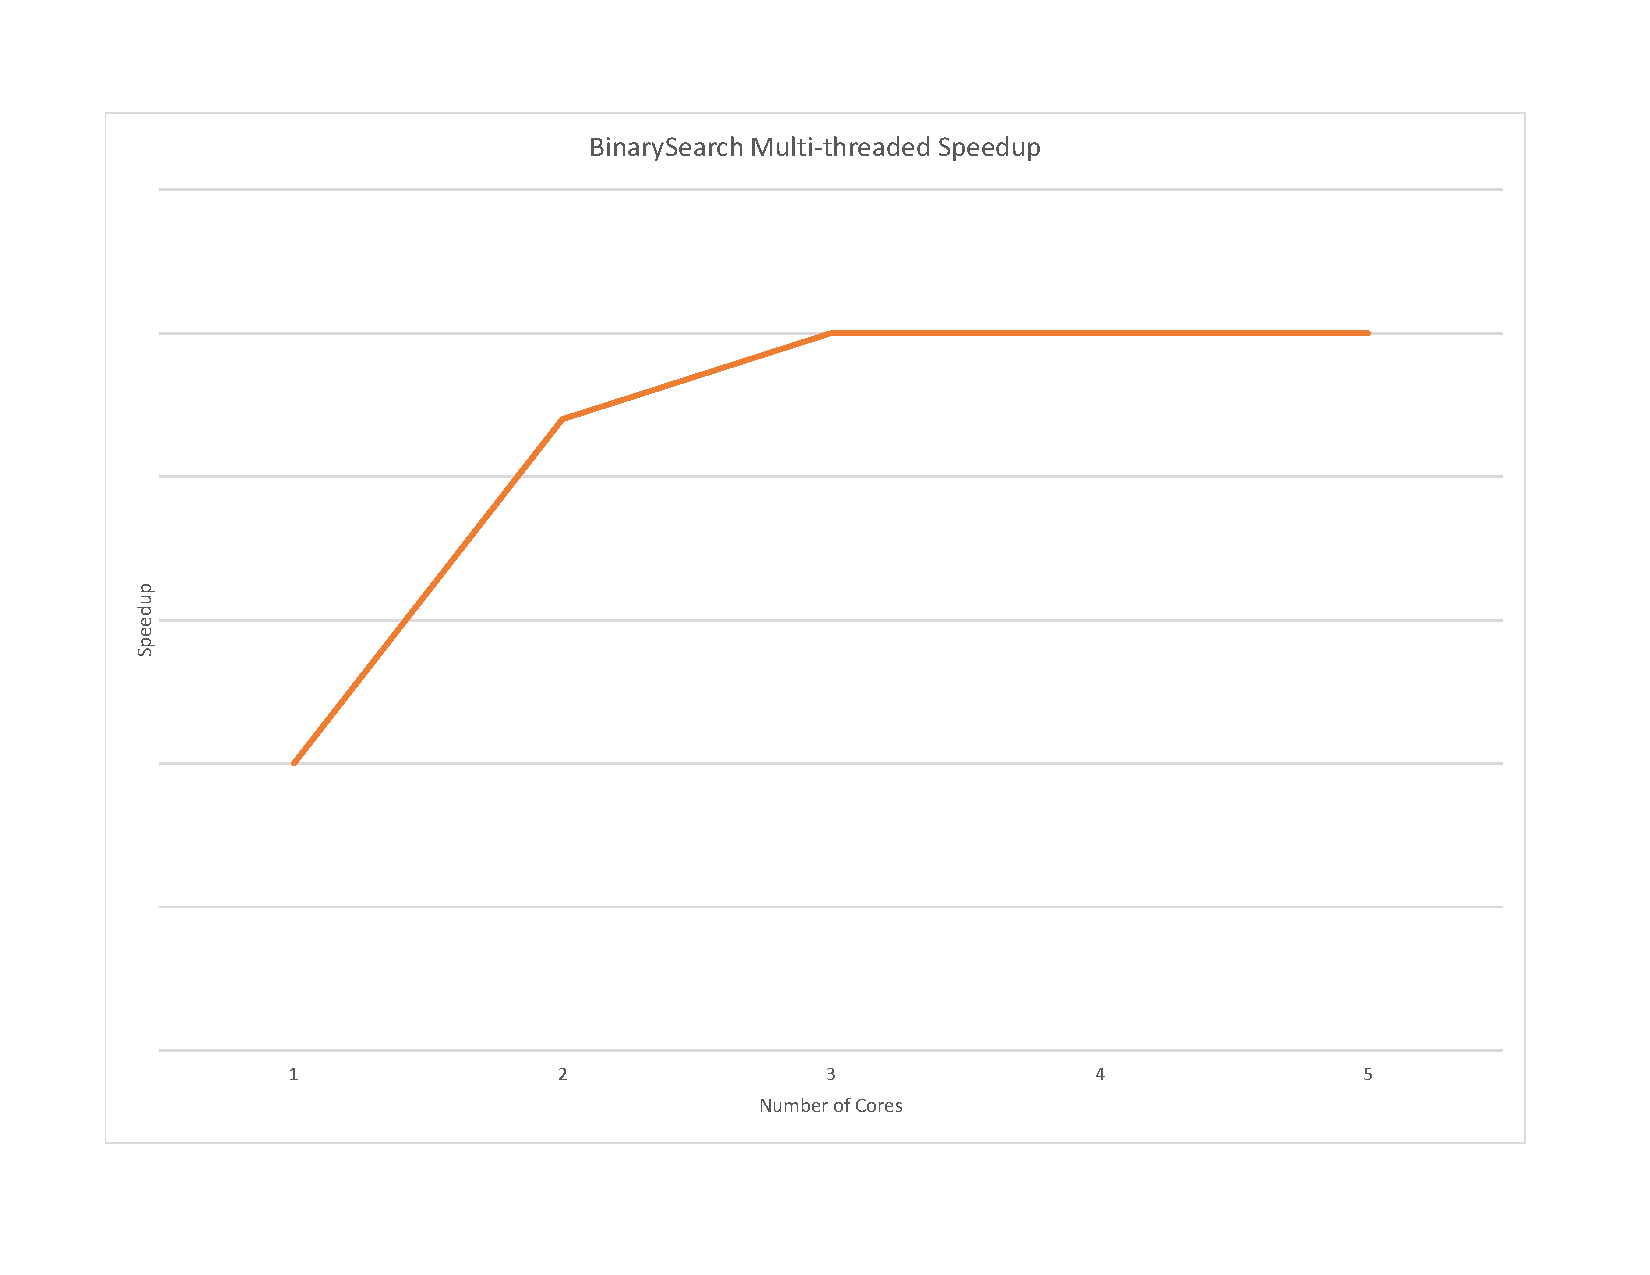
\includegraphics[scale=0.4]{graphs/binarysearch.pdf}
\end{center}

\item
\textbf{6.3.2}

In this problem, we can use the same number of cores as there are elements in the array $A$.  From the previous problem, no noticeable speedup would be observed after the third core based on how the code is constructed.  However, these additional cores could be put to use by creating new threads that would compare the $N$ elements to the given value $X$ in a parallel fashion.  In this case we probably would see a speedup, although we should not forget about any overhead incurred by the instantiation of $N$ threads.  

\end{itemize}

\newpage

\item %2
\textbf{Problem 6.5 from COD reference ($5^{\text{th}}$ Edition).  }

\begin{itemize}

\item
\textbf{6.5.1}

Assuming that $Y$ is much smaller than length($m$), a thread should be spawned for both the left and the right sides of the MergeSort.  Since this is a recursive function, then the number of threads spawned will continue to double until the base two logarithm of $m$ is reached.  This will look something like $1 + 2 + 4 + 8 + \log_2 m$.  

\begin{center}
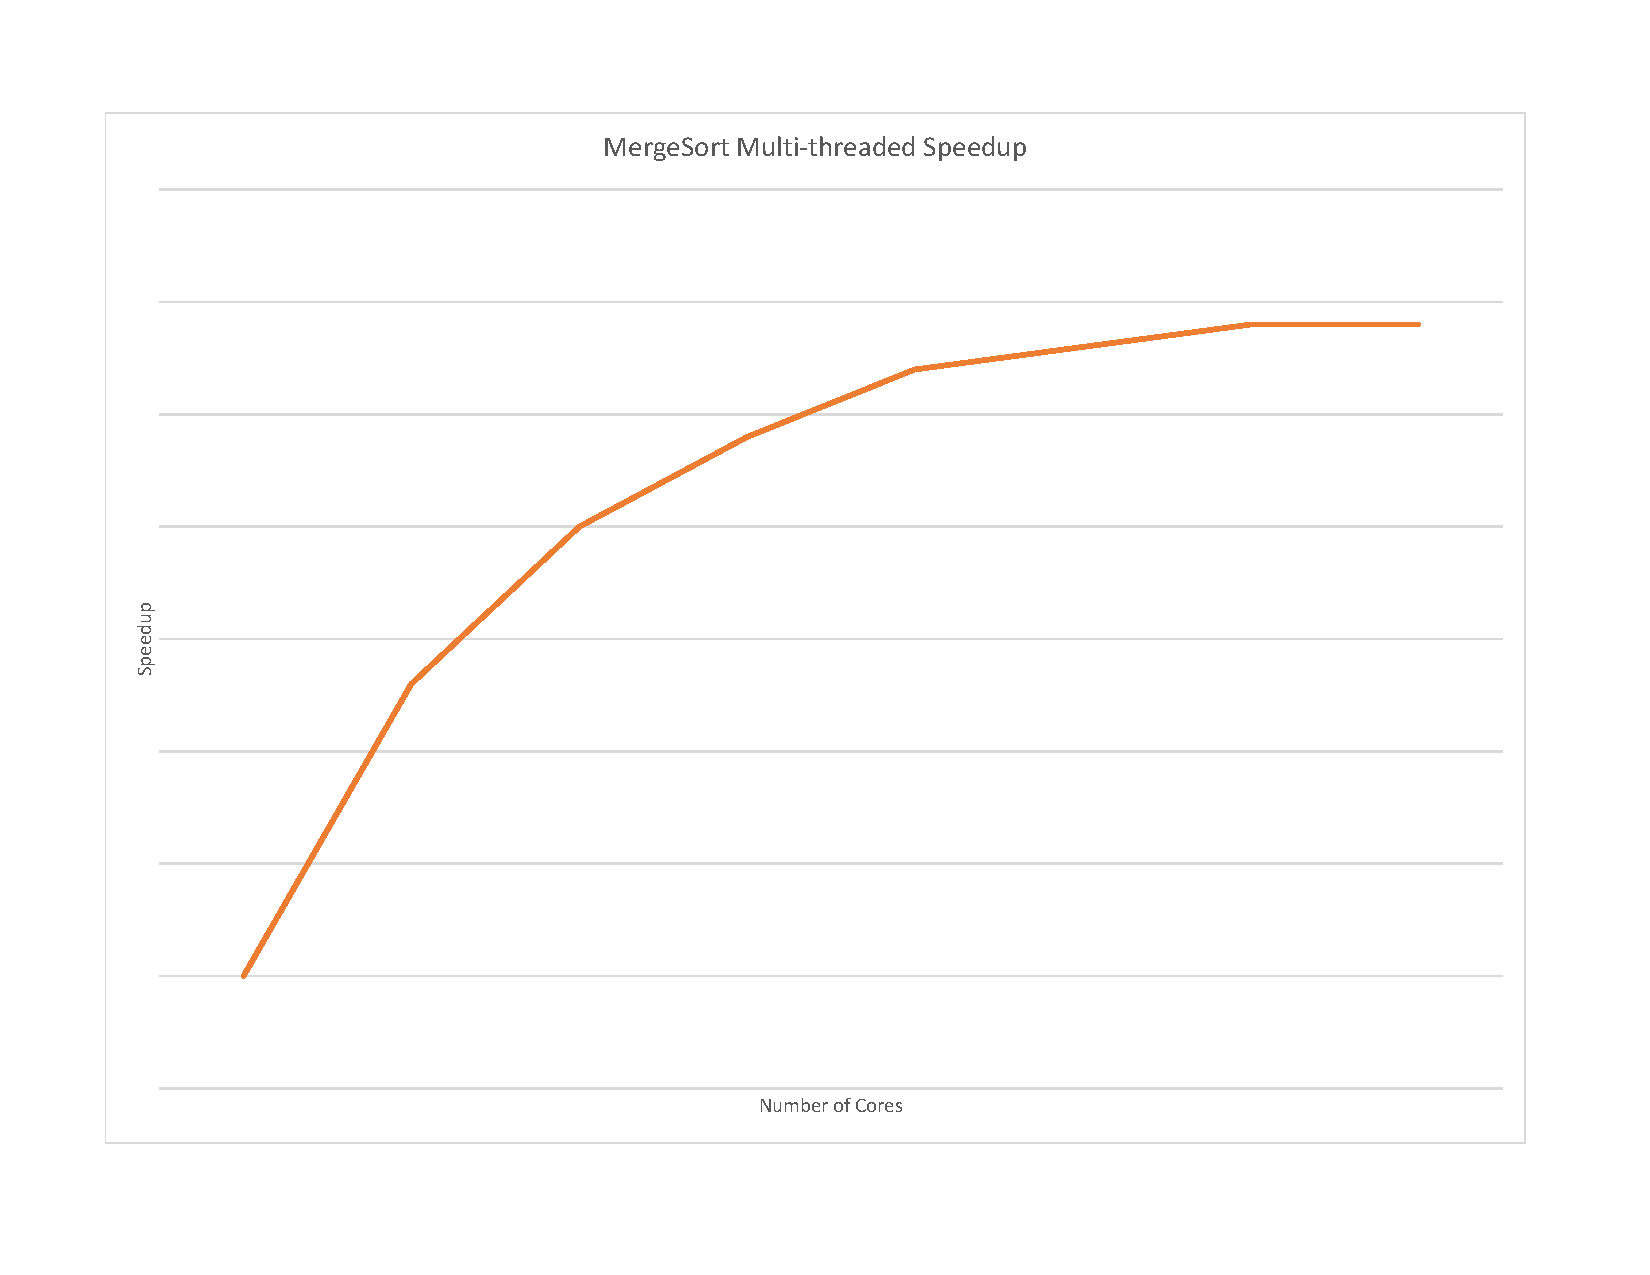
\includegraphics[scale=0.4]{graphs/mergesort.pdf}
\end{center}

\item
\textbf{6.5.2}

If $Y$ is equal to the length($m$), then $\log_2 m$ is the largest value of $Y$ for which we can obtain any speedup based on how the code is structured in part 1.  However, in this case since we have $m$ cores at our disposal, an entirely different algorithm could be used instead of MergeSort.  For example, a different algorithm might compare all pairs of elements in the list and swap the necessary ones so that the right value is greater than the left.  This operation would then be repeated $m$ times so that the list would be fully sorted.  

\end{itemize}

\end{enumerate}
\end{document}






























